\section{Discusión}
\label{sec:discusion}

% ---------------------------------------------------------------
\subsection{La maquinaria transactiva funciona con ocho dominios; la representación es el límite}
\label{sec:disc-escala}

El resultado central separa dos responsabilidades: la maquinaria transactiva funciona
con ocho dominios, y los límites aparecen en la \emph{representación}.
Los componentes de la maquinaria (los directorios heteroasociativos, la lectura B1, el
rechazo por contención, la actualización perspectival del directorio (en imagen) y la
coordinación punto a punto) funcionan sin ajustes por dominio.
En imagen, el registro completo de percepciones de la fase A queda balanceado
(3.000 bits, el máximo con ocho módulos), y los directorios visuales de los módulos
enrutan las imágenes de prueba con dos falsos enrutamientos en 656
(Sección~\ref{sec:hemisferio-visual}).
En texto, las pistas se cuantizan por magnitud sobre una escala global
(Sección~\ref{sec:pipeline-semantico}), que puebla los 16 niveles del alfabeto (una
binarización por signo usaría 2), y con esa representación la precisión temprana sobre
el banco de 411 consultas es del 90.0\%.
Lo que la representación no quita es el solapamiento entre dominios: la
Figura~\ref{fig:espacio-semantico} muestra que persiste, porque es propiedad del léxico
(tres frutas, tres animales), y en él cae la mayoría de los errores que quedan
(Sección~\ref{sec:disc-dominancia}).

\begin{figure}[H]
    \centering
    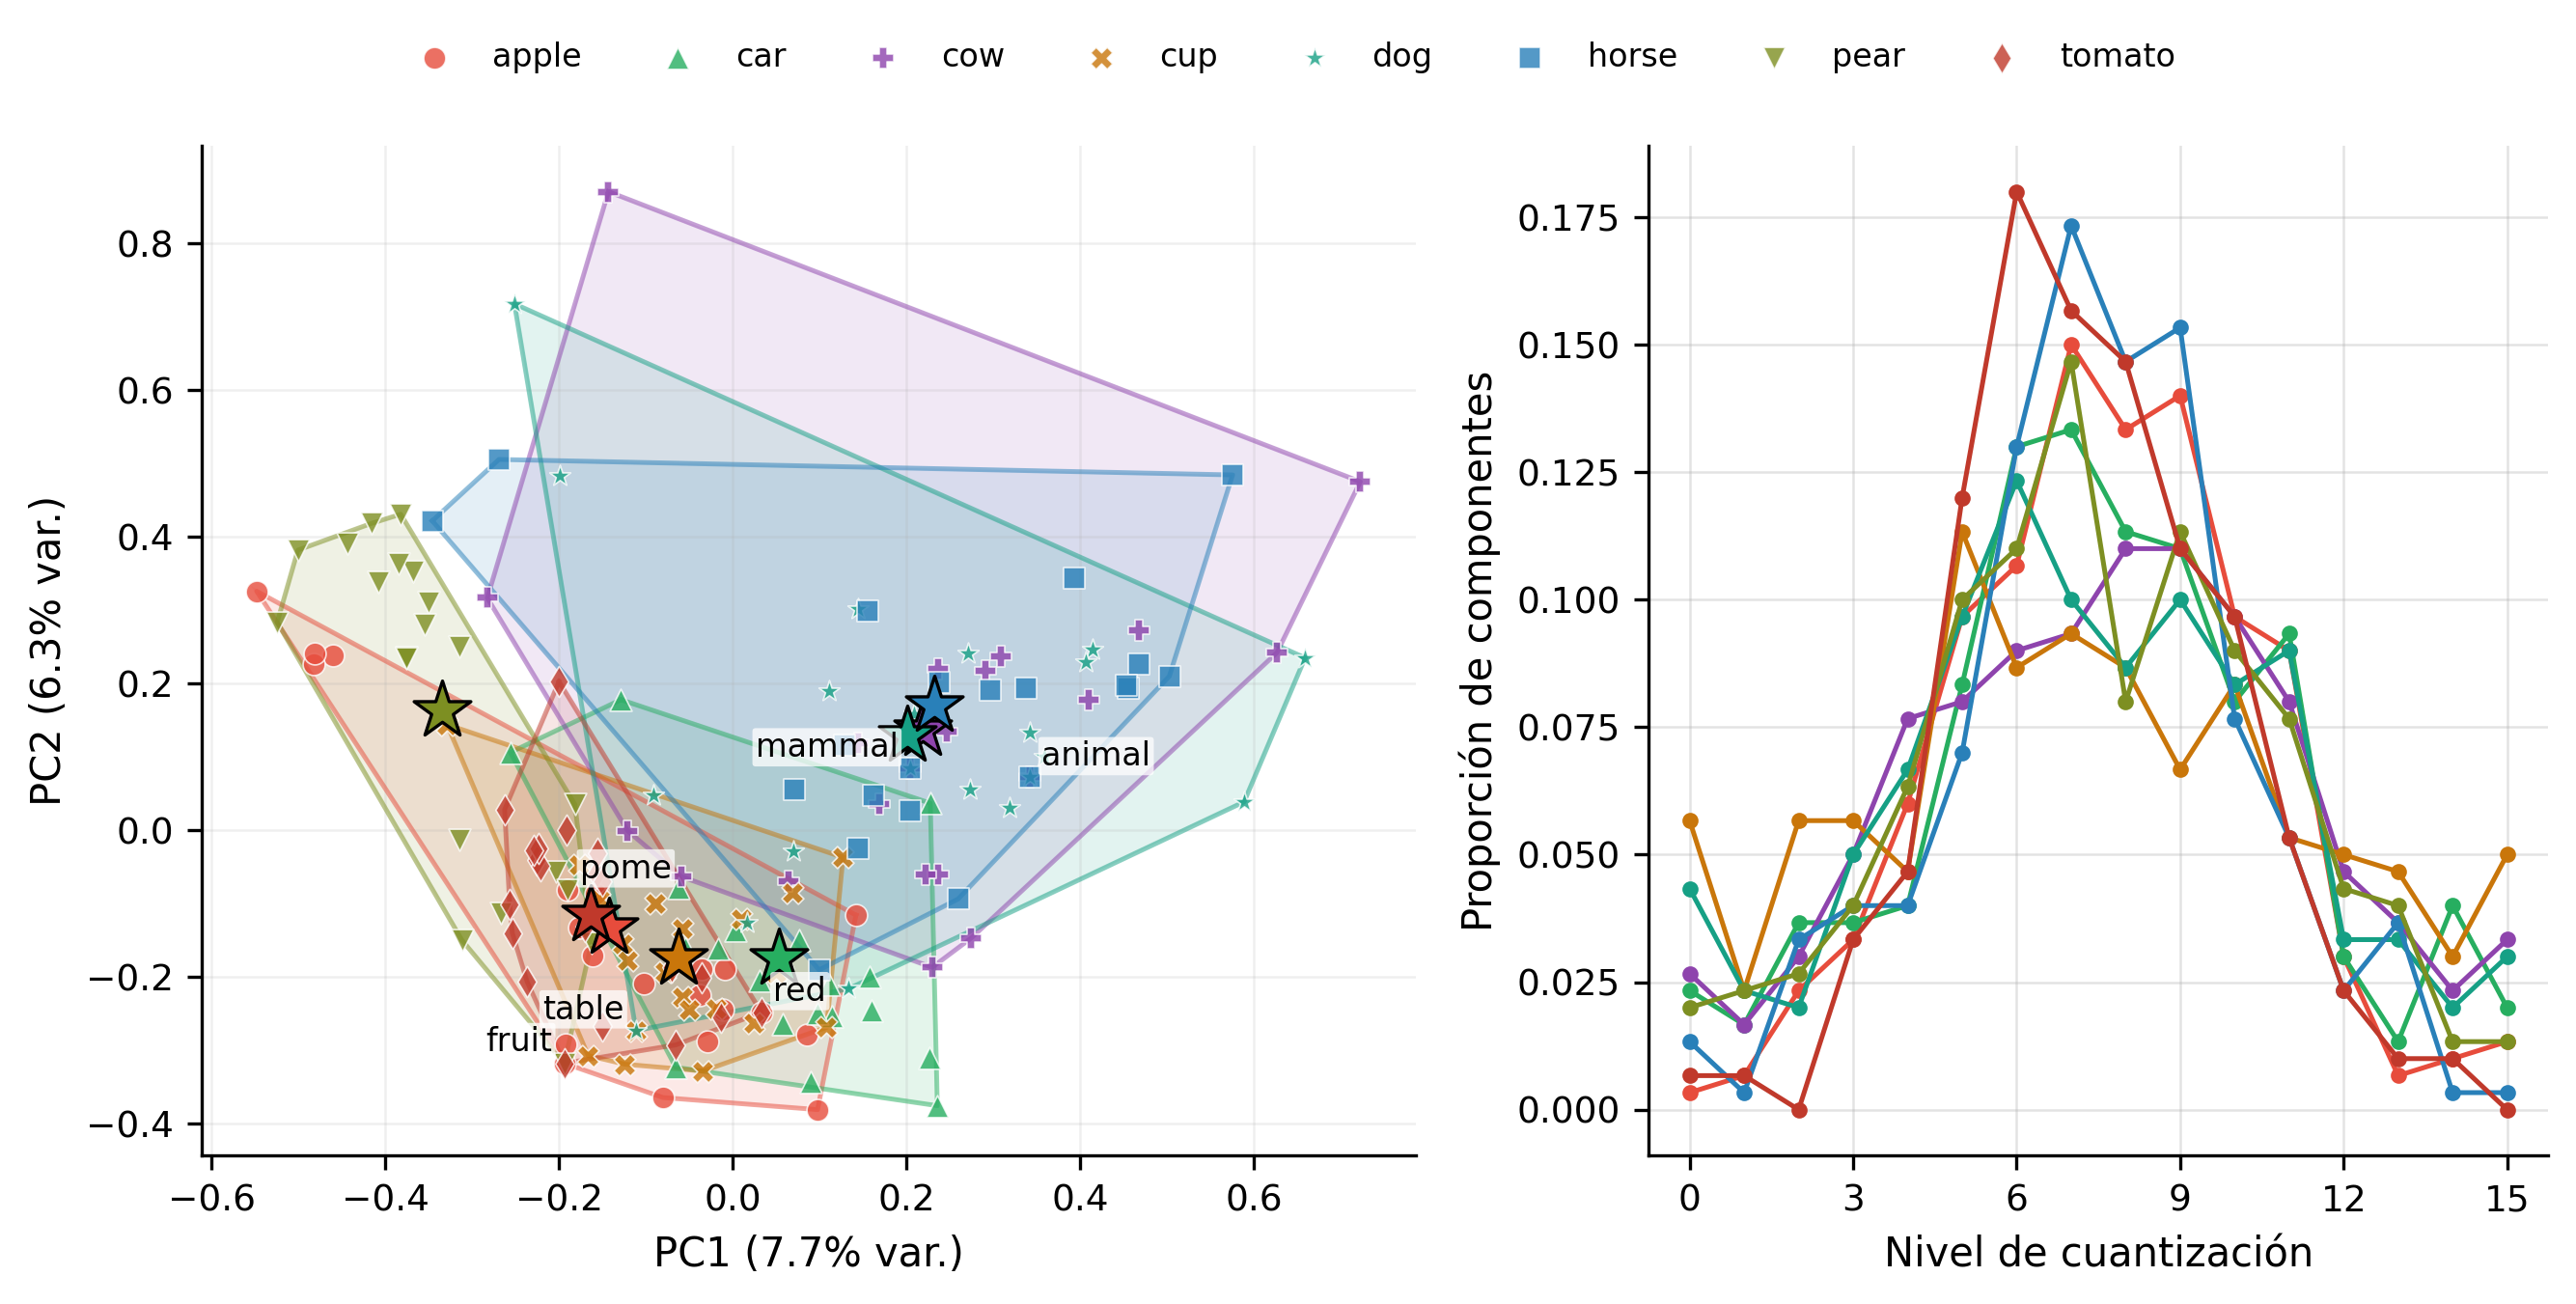
\includegraphics[width=\textwidth]{fig11_semantic_space.png}
    \caption{Espacio semántico de las etiquetas de llenado de las ocho clases (vectores
    fastText del vocabulario de la Sección~\ref{sec:pipeline-semantico}).
    Izquierda: proyección PCA 2D, con la envolvente y el centroide (estrella) de cada
    clase; se rotulan solo las etiquetas que comparten dos o tres clases (\textit{fruit},
    \textit{pome}, \textit{red}, \textit{animal}, \textit{mammal} y \textit{table}).
    Derecha: proporción de las 300 componentes que cae en cada uno de los 16 niveles de
    la cuantización por magnitud, para la etiqueta con el nombre de cada clase.}
    \label{fig:espacio-semantico}
\end{figure}

% ---------------------------------------------------------------
\subsection{La normalización necesaria es B1}
\label{sec:disc-b1}

La lectura B1 del directorio transactivo no corrige un defecto: refleja cómo está
construido el sistema.
Cuando los módulos especialistas acumulan números desiguales de interacciones, la
puntuación cruda del directorio favorece de forma constante al módulo más activo con
independencia del contenido semántico de la consulta.
Dividir entre el conteo normaliza la evidencia a \textit{evidencia por interacción},
comparable entre módulos con historiales de exposición distintos.

La brecha cruda-B1 es de 7.8 puntos con ocho módulos (85.2\% frente a 93.0\%), y la
entropía del directorio es alta incluso con la lectura cruda (2.974 de 3.000 bits): la
\emph{estructura} del directorio está casi balanceada, y el sesgo está en la
\emph{lectura}, donde B1 actúa.
Las condiciones que actúan sobre los síntomas (B2, C, D, E) quedan por debajo de B1, y
la combinación G, que suma correcciones a B1, gana solo medio punto, dentro del ruido
(Tabla~\ref{tab:calibracion}).

% ---------------------------------------------------------------
\subsection{El sesgo hacia un módulo: masa del directorio y léxico compartido}
\label{sec:disc-dominancia}

Con la lectura cruda, \texttt{apple} gana el 20.5\% de las victorias maduras y
\texttt{cow} el 17.0\%: son los dos módulos con más registros en el directorio (186 y
181, frente a 112 de \texttt{horse}).
La puntuación cruda favorece al que más registró (Sección~\ref{sec:disc-b1}); la
lectura B1, que divide entre los registros, deja a \texttt{apple} en 13.8\% (ideal
12.5\%).
Lo que B1 no corrige es léxico.
De los 28 errores que quedan, 9 son \texttt{pear} $\to$ \texttt{apple} y 6
\texttt{horse} $\to$ \texttt{cow}, pares que comparten etiquetas genéricas
(\textit{fruit} y \textit{pome}; \textit{animal} y \textit{mammal}), y \texttt{pear}
se queda en 76\%.
Si el espacio latente del codificador contribuye también al sesgo no se midió en este
trabajo.

% ---------------------------------------------------------------
\subsection{Lectura desde la teoría de memoria transactiva de Wegner}
\label{sec:disc-wegner}

Los resultados de las Secciones~\ref{sec:calibracion}, \ref{sec:formacion},
\ref{sec:capacidad} y~\ref{sec:hemisferio-visual} releen los mecanismos de
Wegner~\cite{wegner1987transactive} con un grupo de ocho miembros:

\begin{itemize}
    \item \textbf{Conocerse cuesta interacción.}
    Con ocho módulos, 10 consultas por dominio dejan la precisión madura en 81.2\%, y
    hace falta el banco completo ($\approx$50 por dominio) para alcanzar el 93.0\%.
    Los errores que quedan caen dentro de pares de módulos que comparten léxico, como
    muestra el punto sobre la comunicación distintiva.

    \item \textbf{El orden de las experiencias afecta la velocidad, no el destino.}
    Todas las condiciones de presentación convergen al mismo directorio: mismos
    conteos, misma entropía.
    En el modelo de Wegner, el directorio se forma anotando quién respondió en cada
    interacción presenciada; aquí cada anotación se suma a las anteriores, así que el
    directorio final depende de \emph{qué} se presenció, y el orden solo decide cuándo
    se vuelve utilizable.

    \item \textbf{La comunicación distintiva forma mejor directorio.}
    Con la lectura B1, \texttt{car}, \texttt{cow}, \texttt{cup} y \texttt{tomato}
    quedan en 98--100\% y \texttt{dog} en 93.9\%; \texttt{pear} (76\%), \texttt{horse}
    (88\%) y \texttt{apple} (88.2\%) pierden hacia la vecina con la que comparten
    etiquetas (Sección~\ref{sec:disc-dominancia}).
    En términos de Wegner, la coordinación de la recuperación funciona en la medida en
    que quien pregunta aporta las señas del dominio: la regla de rescate léxico, que
    solo admite tokens de la consulta como \textit{bark}, \textit{moo} o
    \textit{riding}, sube 21.7 puntos en las 46 consultas que toca
    (Sección~\ref{sec:pipeline-semantico}).

    \item \textbf{El rechazo colectivo se sostiene con ocho dominios.}
    Con siete clases contrarias por módulo, el contenido no acepta ningún falso con un
    latente por imagen, en ninguno de los tamaños de llenado probados, y con las 16
    variantes del experimento 13 acepta 5 de 656 imágenes de prueba, todas entre
    animales (vacas y caballos aceptados por \texttt{dog}, un caballo por
    \texttt{cow}).
    El directorio visual comete dos falsos enrutamientos de 656.
    Es el rechazo de la Sección~\ref{sec:tmt}: lo que ningún módulo reconoce no se
    responde, y los falsos del contenido caen entre animales.
\end{itemize}

% ---------------------------------------------------------------
\subsection{Una memoria por módulo: familiaridad, nombre y daño}
\label{sec:disc-una-memoria}

Con una sola memoria de contenido, el sistema queda hecho solo de asociaciones: la de
contenido (etiqueta con imagen) dentro de cada módulo y la de directorio (pista con
módulo) entre ellos.
Reconocer una pista no consulta un almacén aparte: es leer la asociación.
Es lo que proponen los modelos de emparejamiento global de la psicología, que leen la
familiaridad de un único almacén de huellas~\cite{clark1996global}: preguntarle a la
memoria conjunta si una imagen es familiar es emparejarla con todas las huellas,
cualquiera que sea su etiqueta, y eso es la suma de la ecuación~\eqref{eq:marginal}.

La lesión de la Sección~\ref{sec:una-memoria} separa las dos lecturas: con daño al
azar en la única memoria, el módulo deja de nombrar mucho antes de dejar de reconocer
(Tabla~\ref{tab:lesion}).
El patrón se parece a disociaciones conocidas.
La paciente YR, con una lesión selectiva del hipocampo, reconoce ítems pero falla en
asociaciones entre tipos distintos de información, como caras con nombres
hablados~\cite{mayes2004associative}.
En ratas, la lesión del hipocampo suprime el recuerdo y deja la
familiaridad~\cite{fortin2004recollection}; con la edad, la memoria de asociaciones se
deteriora más que la de ítems~\cite{old2008differential}.
En el cerebro, estas disociaciones suelen atribuirse a estructuras distintas, la corteza
perirrinal para la familiaridad y el hipocampo para unir ítem y
contexto~\cite{eichenbaum2007medial,diana2007imaging}, aunque esa asignación está en
disputa~\cite{squire2007recognition}.
En este sistema la disociación sale de una sola memoria: nombrar exige que cada
coordenada de la imagen deje apoyo en cada coordenada de la etiqueta, mientras que
reconocer suma la evidencia de todas las etiquetas.
Esto no resuelve el debate, pero muestra que la disociación no exige dos almacenes, como
Plaut mostró para la afasia óptica con un solo sistema semántico de especialización
gradual~\cite{plaut2002graded}.

El estado intermedio, reconocer sin poder nombrar, también tiene análogos.
En la afasia óptica, el paciente identifica un objeto por la vista pero no puede
nombrarlo desde ella~\cite{beauvois1982optic}.
En la experiencia de la punta de la lengua, la persona sabe que conoce la palabra y
recupera partes de ella, como la primera letra o el número de sílabas, sin
alcanzarla~\cite{brown1966tip}; y la sensación de saber anticipa con bastante acierto qué
se reconocerá aunque no se haya podido recordar~\cite{hart1965memory}.
En este sistema el estado aparece en cuanto hay datos sin pareja: de 800 imágenes
registradas sin palabra, 78 quedan reconocidas sin nombre (Sección~\ref{sec:una-memoria}).
La lectura de familiaridad las distingue de un rechazo; el protocolo de respuesta
todavía no las usa.
En términos de Wegner~\cite{wegner1987transactive}, es justo el momento en que un miembro
del grupo debería consultar el directorio: sabe que conoce el objeto y necesita a quien
sepa el nombre.
Estas analogías son estructurales, no causales: en los pacientes la asociación existía y
se dañó; en el sistema, con datos sin pareja, nunca se registró.

% ---------------------------------------------------------------
\subsection{Qué aporta la partición frente a una EHAM única}

La comparación de la Sección~\ref{sec:eham-unica} acota lo que aporta la maquinaria
transactiva.
Lo primero es no mezclar: la relación de una EHAM acumula por coordenada y valor, y dos
conceptos distintos comparten valores cuantizados en muchas coordenadas, así que una
memoria con varios dominios mezcla al recordar aunque las palabras difieran.
Partir el contenido evita la mezcla porque el dominio se decide antes de la
recuperación, en el directorio, y no al muestrear la memoria.
Se ve en la fidelidad: la respuesta de la EHAM única queda más lejos de la instancia
real más cercana en todos los cortes (de 4.6 a 6.2 más que el oráculo), sin tendencia
con el contenido.
Y se ve fuera de dominio: la EHAM única acepta más cuanto más contiene (de 2 a 8 de 40
consultas), y el protocolo con doble compuerta acepta 2 en todos los cortes.

La exactitud de clase también mejora, pero poco.
Desde 50 imágenes por clase el protocolo acierta entre 98.3 y 98.8\,\% frente a
96.9--97.6\,\% de la EHAM única, con intervalos separados; con 25 la EHAM única queda
arriba (97.6 frente a 96.9\,\%, con intervalos que se solapan), porque el directorio
todavía enruta peor (95.3\,\% de enrutamiento correcto).

El precio es cobertura y un índice.
El especialista deja sin respuesta al 2.5\,\% de las imágenes de prueba con 200 por
clase, que la EHAM única responde: una de las 80 imágenes porque la contención es
estricta en las 64 coordenadas del latente y otra porque el recuerdo no devuelve palabras.
Es parte del rechazo residual del hemisferio visual (limitación (b)); el protocolo de
esta comparación, que forma su directorio visual sin variantes, responde al 81\,\%.
A eso se suman el error del directorio, de 1.2 a 1.7 puntos de clase desde 50 imágenes
por clase (3.1 con 25), y ocho veces las celdas de memoria: una heteroasociativa por
módulo en lugar de una.

\subsection{Limitaciones}
\label{sec:limitaciones}

\paragraph{(a) Fuga de consultas fuera de dominio en el hemisferio textual.}
Una consulta fuera de dominio que comparte tokens con etiquetas legítimas pasa la
contención textual y llega a algún módulo: la sonda de rechazo deja pasar 2 de 12
(Sección~\ref{sec:proto-completo}), y en el banco de 40 de la comparación con la EHAM
única el directorio acepta 4, dos de ellas (\emph{piano}, \emph{thunderstorm}) hacia un
módulo que no las contiene.
La doble compuerta de contenido (el destino debe contener la consulta, no solo figurar
en el directorio) detiene esas dos y deja al protocolo en 2 de 40 en los cuatro cortes,
tantas como el oráculo; sobre las 171 consultas reservadas no quita ninguna respuesta,
porque las que rechaza (1.5\,\% con 200 imágenes por clase, 2.1\,\% con 25) eran
enrutamientos equivocados que el destino tampoco respondía.
Las dos que quedan las contiene el destino, y ninguna compuerta de contención las
separa de una consulta legítima.
Las alternativas medidas rinden menos (experimento 15, sobre las 171 reservadas): que el
contenido decida entre los tres mejores candidatos del directorio baja el acierto de
96.8 a 93.6\,\%, porque el índice calibrado compara mejor que la activación del
contenido, y abstenerse cuando la diferencia relativa entre las dos mejores
puntuaciones es menor que un umbral $\delta$ quita más de un acierto por cada error
evitado (1.2 con $\delta = 0.05$; 8 con $\delta = 0.5$).

\paragraph{(b) Cobertura visual limitada por la lectura estricta.}
La lectura del directorio visual es estricta ($\xi = 0$): con directorios
perspectivales, los huecos tolerados dependerían de lo que presenció cada módulo.
Para cubrir más, el sistema densifica.
El directorio visual y la recuperación de la heteroasociativa son dos compuertas, y
cada una cede solo con sus propias variantes (experimento 13, sobre las 656 imágenes de
prueba): registrar en el directorio 16 variantes por percepción, en lugar de una, lleva
su aceptación de 73.6 a 96.2\,\%; llenar el contenido con 16 variantes por imagen, en
lugar de 4, lleva la respuesta de la heteroasociativa de 76 a 96\,\%; con las dos, la
cobertura de punta a punta (enrutamiento correcto y respuesta) pasa de 66.5 a
94.5\,\%, con rendimiento decreciente por escalón de variantes.
El sistema usa 16 variantes en las dos y aun así rechaza el 3.5\,\% de las imágenes de
prueba (Sección~\ref{sec:hemisferio-visual}).
Densificar tiene un costo: dos enrutamientos equivocados de 656 y, en el experimento,
cinco imágenes aceptadas por un especialista ajeno, todas entre animales y cuatro de
ellas por \texttt{dog}.
Son vistas nuevas de los mismos objetos, porque la partición es por imagen
(limitación (f)).

\paragraph{(c) Fuga con entradas degeneradas.}
El contenido visual da soporte también a entradas sin estructura, como un lienzo gris
uniforme, porque el codificador las lleva a latentes de norma baja que caen dentro de la
envolvente de los animales (Sección~\ref{sec:hemisferio-visual}); las sondas
estructuradas (ruido, píxeles barajados) sí se rechazan.
Densificar agranda esa fuga: en el experimento 13, con 16 variantes, a la sonda de color
sólido la aceptan tres especialistas en vez de uno y el directorio la enruta.
El umbral de energía (Sección~\ref{sec:percepcion}) cierra el 90\,\% de la fuga
(experimento 14): 137 de las 152 entradas degeneradas aceptadas por una clase ajena caen
bajo $\tau$ (grises de 104 a 168, contrastes $\leq 0.2$ y desenfoques fuertes: todos
los de radio $\geq 12$ y buena parte de los menores).
Como criterio, la norma y la varianza del latente son equivalentes; la varianza de
píxeles no sirve, porque un objeto desenfocado conserva contraste y pierde estructura.
De las 15 entradas que sobreviven, 11 son objetos desenfocados o de bajo contraste que
acepta otra clase (como un \texttt{dog} desenfocado aceptado por \texttt{cow}) y cuatro
son superficies casi uniformes de norma alta (un gris claro, dos colores sólidos y un
gris con ruido); la doble compuerta del punto (a) no las cerraría, porque el contenido
también las acepta.
El umbral cuesta cinco imágenes reales de 3280, todas vistas oscuras de \texttt{cow}:
una percepción de la fase A y cuatro imágenes de prueba que el directorio enrutaba bien
y su contenido aceptaba.

\paragraph{(d) Calidad de la reconstrucción visual.}
Las reconstrucciones son suaves y sin detalle de alta frecuencia
(Figura~\ref{fig:imagen-etiquetas}).
Es un efecto de cómo se entrenó el autocodificador, con un término de reconstrucción MSE y
una cabeza auxiliar de clasificación que solo interviene en el entrenamiento, no en las
decisiones; no es un efecto del sistema de memorias y puede abordarse por separado.
Sobre la reconstrucción en la EAM, véanse la imaginería de Pineda y
Morales~\cite{pineda2023imagery} y la memoria de imágenes naturales de
CIFAR-10~\cite{hernandez2026cifar}, donde entrenar el autocodificador junto con el
clasificador degrada la reconstrucción y por eso se entrenan por separado.

\paragraph{(e) Aprendizaje limitado después de formar el directorio.}
Una vez llena la memoria de contenido y formado el directorio, los módulos dejan de
registrar contenido nuevo: la fase madura enruta y recupera con lo aprendido.
El sistema aún no modela la asignación de información de Wegner (encaminar información
nueva al especialista que corresponde) ni la reorganización de las memorias de contenido
durante la operación madura.

\paragraph{(f) Partición por imagen.}
La partición entre entrenamiento y prueba separa archivos de imagen, no objetos
físicos: los diez objetos de cada clase aportan vistas a ambos lados
(Sección~\ref{sec:dataset}).
Las cifras visuales principales (96.2\% de enrutamiento, evocación de dominio) miden por
tanto generalización a \emph{vistas nuevas de objetos conocidos}.
Con objetos nuevos, la cobertura de punta a punta baja del 95.5 al 89.2\,\%
(Sección~\ref{sec:objetos-nuevos}), y lo que se pierde es respuesta, no acierto: la
envolvente por coordenada cubre a la mayoría de los objetos que no contribuyeron a ella,
rechaza las vistas que no cubre en lugar de enviarlas a otra clase, y la brecha se
concentra en unos pocos objetos, no en clases.
Con diez objetos por clase, ``objeto nuevo'' sigue siendo un objeto de la misma
colección fotografiado en las mismas condiciones; fotos de otro origen son otra
pregunta.

\paragraph{(g) Selección de modelo e hiperparámetro sobre el conjunto de prueba.}
Dos elementos del protocolo se eligieron mirando el conjunto de prueba, por ausencia
de una partición de validación separada: el punto de control del codificador (RMSE
mínimo sobre el conjunto de prueba entre cinco candidatos, Sección~\ref{sec:percepcion})
y las 16 variantes del llenado, adoptadas después de ver el barrido de variantes
(experimento 13), que mide sobre las 656 imágenes de prueba (16 es el mayor valor
probado, no un óptimo ajustado).
La lectura del directorio visual no tiene tolerancia que ajustar ($\xi = 0$,
limitación (b)).
Ambas selecciones son de alcance acotado y ninguna introduce un mecanismo ajeno a las
memorias, pero pueden inflar las cifras visuales reportadas; la corrección (una
partición de validación aparte) es directa y queda pendiente.

\paragraph{(h) Regla de admisión de pistas alineada con el vocabulario propio.}
El rescate de atención léxica (Sección~\ref{sec:pipeline-semantico}) admite tokens
que el filtro gramatical (POS) descarta si figuran en el vocabulario que llenó las
memorias; su efecto medido es de +21.7 puntos sobre las 46 consultas afectadas del
banco (43 de 46 correctas con rescate, 33 sin él).
La regla nunca censura y no decide el ganador, pero decide \emph{quién vota} con un
criterio derivado del conocimiento del propio sistema; un criterio de rescate
independiente del vocabulario (p.\ ej.\ solo la etiqueta POS de diccionario) eliminaría
la alineación al costo medido.

\paragraph{(i) Dependencia de la calidad de la fuente de conocimiento.}
El vocabulario de ConceptNet es asimétrico entre clases, y el techo de las clases de
léxico compartido (\texttt{pear} 76\%, \texttt{horse} 88\%) depende de la
distintividad de las consultas del banco tanto como del vocabulario del módulo.
Este trabajo no midió si enriquecer el vocabulario de una clase lo corrige.

\paragraph{(j) Fragilidad del nombre ante daño.}
La proyección exige que cada coordenada de la imagen deje apoyo en cada coordenada de la
etiqueta, y no tolera ninguna columna vacía.
Destruir al azar el 1\,\% de las celdas de la memoria de contenido deja sin nombre al
92\,\% de las imágenes emparejadas, y el 5\,\% a todas
(Tabla~\ref{tab:lesion}); el reconocimiento, en cambio, sobrevive.
